\documentclass{beamer}

% Required packages
\usepackage{amsmath}
\usepackage{physics}
\usepackage{graphicx}
\usepackage{siunitx}
\usepackage{xcolor}

% Set image search paths
\graphicspath{{../images/}{../../shared/images/}}

% Define custom colors for DS9 theme
\definecolor{ds9blue}{RGB}{25,25,112}
\definecolor{ds9gold}{RGB}{218,165,32}
\definecolor{ds9grey}{RGB}{105,105,105}
\definecolor{ds9red}{RGB}{178,34,34}

% Set up the Madrid theme with custom colors
\usetheme{Madrid}
\usecolortheme{whale}

\setbeamercolor{palette primary}{bg=ds9blue,fg=white}
\setbeamercolor{palette secondary}{bg=ds9grey,fg=white}
\setbeamercolor{palette tertiary}{bg=ds9gold,fg=black}
\setbeamercolor{palette quaternary}{bg=ds9red,fg=white}
\setbeamercolor{structure}{fg=ds9blue}
\setbeamercolor{title}{fg=ds9gold}
\setbeamercolor{subtitle}{fg=ds9gold}
\setbeamercolor{frametitle}{bg=ds9blue,fg=white}
\setbeamercolor{block title}{bg=ds9blue,fg=white}
\setbeamercolor{block body}{bg=ds9grey!20,fg=black}

% Title information
\title[Electric Potential \& Capacitors]{PHYS12 CH19: Electric Potential and Electric Field}
\subtitle{Electric Potential, Fields, and Capacitors}
\author[Mr. Gullo]{Mr. Gullo}
\date[Feb 2025]{February, 2025}
\institute{Physics Department}

\begin{document}

% Title slide
\begin{frame}
    \titlepage
\end{frame}

% Outline slide
\begin{frame}
    \frametitle{Outline}
    \tableofcontents
\end{frame}

\section{Introduction}

\begin{frame}
    \frametitle{Learning Objectives}
    By the end of this presentation, you will be able to:
    \begin{itemize}
        \item Define electric potential and explain how it relates to potential energy
        \item Calculate potential difference between points in an electric field
        \item Relate electric field strength to potential gradient
        \item Calculate the electric potential due to a point charge
        \item Understand the concept of equipotential lines
        \item Explain how capacitors work and calculate capacitance
        \item Determine the equivalent capacitance of series and parallel combinations
        \item Calculate the energy stored in a capacitor
    \end{itemize}
\end{frame}

\section{Electric Potential Energy and Potential Difference}

\begin{frame}
    \frametitle{Electric Potential Energy vs. Electric Potential}
    
    \begin{block}{Electric Potential Energy}
        \begin{itemize}
            \item Energy possessed by a charge in an electric field
            \item Depends on both the field and the amount of charge
            \item Measured in joules (J)
        \end{itemize}
    \end{block}
    
    \begin{block}{Electric Potential}
        \begin{itemize}
            \item Electric potential energy per unit charge
            \item Independent of the test charge being used
            \item Measured in volts (V), where 1 V = 1 J/C
            \item A property of the electric field at a point
        \end{itemize}
    \end{block}
    
    
\end{frame}

\begin{frame}
    \frametitle{Potential Difference and Voltage}
    
    \begin{block}{Potential Difference}
        \begin{itemize}
            \item The change in potential energy per unit charge when moving from point A to point B
            \item Commonly called voltage
        \end{itemize}
    \end{block}
    
    \begin{align}
        \Delta V &= \frac{\Delta PE}{q} \\
        \Delta PE &= q \Delta V
    \end{align}

    \begin{itemize}
        \item Work must be done to move a positive charge from a low potential to a high potential
        \item A positive charge naturally moves from high potential to low potential (releasing energy)
        \item A negative charge naturally moves from low potential to high potential
    \end{itemize}
\end{frame}

\begin{frame}
    \frametitle{The Electron Volt}
    
    \begin{block}{Definition}
        The electron volt (eV) is the energy given to a fundamental charge accelerated through a potential difference of 1 V.
    \end{block}
    
    \begin{align}
        1 \text{ eV} &= (1.60 \times 10^{-19} \text{ C})(1 \text{ V}) \\
        &= (1.60 \times 10^{-19} \text{ C})(1 \text{ J/C}) \\
        &= 1.60 \times 10^{-19} \text{ J}
    \end{align}
    
    \begin{itemize}
        \item Useful unit for atomic and nuclear physics
        \item Common multiples: keV, MeV, GeV
        \item Example: A 12 V battery can give an electron 12 eV of energy
    \end{itemize}
\end{frame}

\begin{frame}
    \frametitle{Conservation of Energy in Electric Fields}
    
    \begin{block}{Mechanical Energy}
        \begin{itemize}
            \item The sum of kinetic energy and potential energy of a system
            \item $E_{mechanical} = \text{KE} + \text{PE}$
            \item This sum is constant in a conservative field
        \end{itemize}
    \end{block}
    
    \begin{block}{Applications}
        \begin{itemize}
            \item When a charge moves in an electric field, energy is converted between kinetic and potential forms
            \item $\Delta \text{KE} = -\Delta \text{PE} = -q\Delta V$
            \item Can find the final speed of a charged particle accelerated through a potential difference
        \end{itemize}
    \end{block}
\end{frame}

\section{Electric Potential in a Uniform Field}

\begin{frame}
    \frametitle{Electric Potential in a Uniform Field}
    
    In a uniform electric field (like between parallel plates):
    \begin{align}
        V_{AB} &= Ed \\
        E &= \frac{V_{AB}}{d}
    \end{align}
    where:
    \begin{itemize}
        \item $E$ is the electric field strength (V/m or N/C)
        \item $d$ is the distance from A to B (m)
        \item $V_{AB}$ is the potential difference (V)
    \end{itemize}
    \end{frame}

\begin{frame}
    \begin{figure}
        \centering
        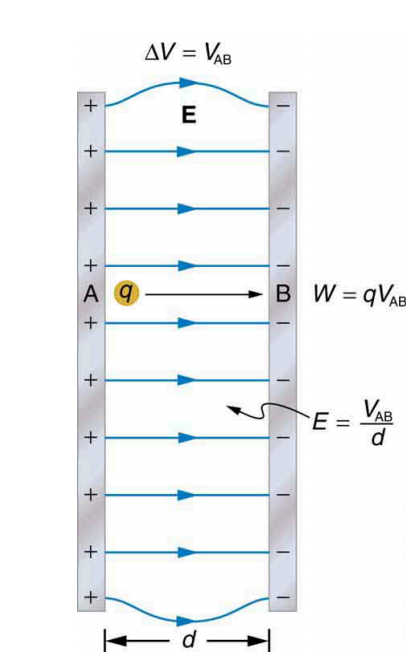
\includegraphics[width=0.4\linewidth]{phys12-electrostatics-parallel-plates-electric-field.png}
        \caption{Fig 19.5}
    \end{figure}
\end{frame}

\begin{frame}
    \frametitle{Relationship Between Electric Field and Potential}
    
    \begin{block}{General Relationship}
        \begin{align}
            E &= -\frac{\Delta V}{\Delta s}
        \end{align}
        where $\Delta s$ is the distance over which the change in potential $\Delta V$ takes place
    \end{block}
    
    \begin{itemize}
        \item The negative sign indicates that E points in the direction of decreasing potential
        \item Electric field is the gradient (slope) of the electric potential
        \item Units check: $\text{V/m} = \text{N/C}$
        \item Stronger electric fields create steeper potential gradients
    \end{itemize}
\end{frame}

\section{Electric Potential Due to a Point Charge}

\begin{frame}
    \frametitle{Electric Potential Due to a Point Charge}
    
    \begin{block}{Point Charge Potential}
        The electric potential at a distance $r$ from a point charge $Q$ is:
        \begin{align}
            V = k\frac{Q}{r}
        \end{align}
        where $k = 9.0 \times 10^9 \text{ N}\cdot\text{m}^2/\text{C}^2$
    \end{block}
    
    \begin{itemize}
        \item Potential is positive for positive charges and negative for negative charges
        \item Decreases with distance $r$ from the charge
        \item Reference: $V = 0$ at $r = \infty$
        \item Note: $E = k\frac{Q}{r^2}$, so $E = -\frac{dV}{dr}$
    \end{itemize}
\end{frame}

\begin{frame}
    \frametitle{Superposition of Potentials}
    
    \begin{block}{Key Concept}
        Electric potential is a scalar quantity, so potentials from multiple charges add algebraically:
        \begin{align}
            V_{total} = V_1 + V_2 + V_3 + \cdots = \sum_i V_i = k\sum_i \frac{Q_i}{r_i}
        \end{align}
    \end{block}
    
    \begin{itemize}
        \item This is simpler than adding electric fields (which are vectors)
        \item Makes it easier to solve some complex electrostatic problems
        \item Calculate the total potential, then find the electric field by taking the gradient
    \end{itemize}
\end{frame}

\section{Equipotential Lines}

\begin{frame}
    \frametitle{Equipotential Lines and Surfaces}
    
    \begin{block}{Definition}
        An equipotential line is a line along which the electric potential is constant.
    \end{block}
    
    \begin{itemize}
        \item An equipotential surface is the 3D version of equipotential lines
        \item No work is done moving a charge along an equipotential
        \item Equipotential lines are always perpendicular to electric field lines
        \item For a point charge, equipotentials are concentric spheres
        \item For a uniform field, equipotentials are parallel planes
    \end{itemize}
\end{frame}

\begin{frame}{}
    

\begin{figure}
    \centering
    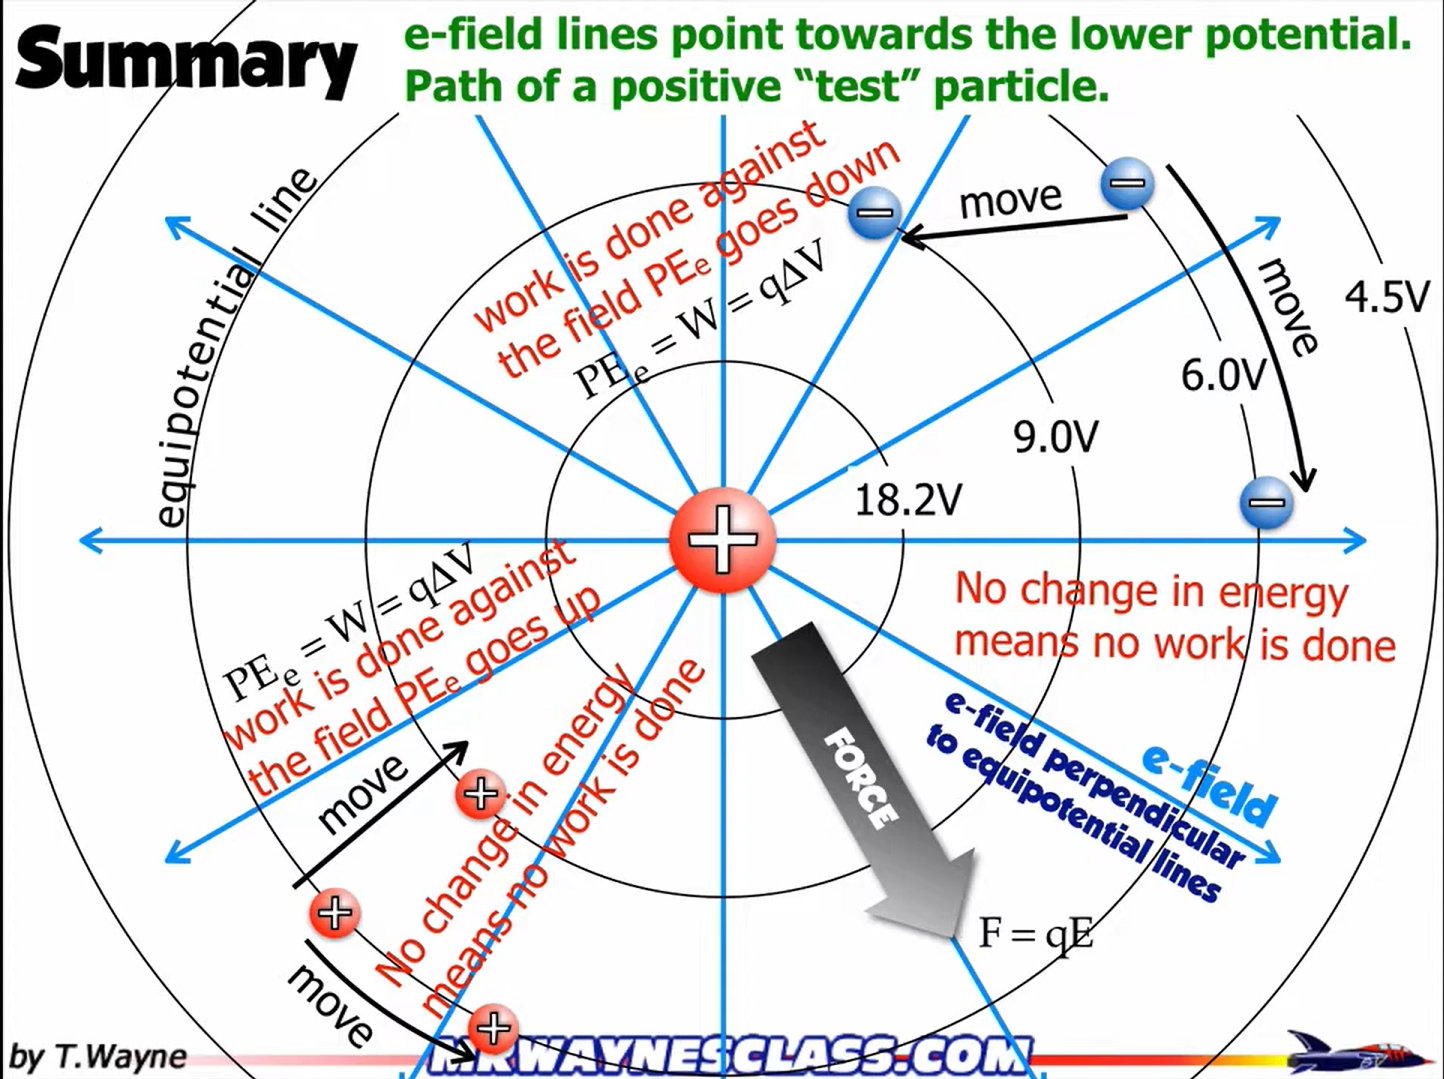
\includegraphics[width=0.75\linewidth]{phys12-electrostatics-equipotential-lines.png}
\end{figure}
\end{frame}

\begin{frame}
    \frametitle{Equipotential Lines and Grounding}
    
    \begin{block}{Properties of Equipotentials}
        \begin{itemize}
            \item All points on a conductor in electrostatic equilibrium are at the same potential
            \item The surface of a conductor is an equipotential surface
            \item No electric field exists inside a conductor in electrostatic equilibrium
        \end{itemize}
    \end{block}

    
    \begin{block}{Grounding}
        \begin{itemize}
            \item Grounding is the process of connecting a conductor to the Earth with a good conductor
            \item This fixes the conductor at zero volts (Earth's reference potential)
            \item Important for safety in electrical systems
        \end{itemize}
    \end{block}
\end{frame}

\section{Capacitors and Dielectrics}

\begin{frame}
    \frametitle{What is a Capacitor?}
    
    \begin{block}{Definition}
        A capacitor is a device used to store electric charge and energy in an electric field.
    \end{block}
    
    \begin{itemize}
        \item Typically consists of two conductors (plates) separated by an insulator (dielectric)
        \item When connected to a voltage source, equal and opposite charges appear on the conductors
        \item The electric field is confined mostly to the region between the conductors
        \item Common forms: parallel plate, cylindrical, spherical
    \end{itemize}
    \end{frame}

\begin{frame}{Capacitors}
    \begin{figure}
        \centering
        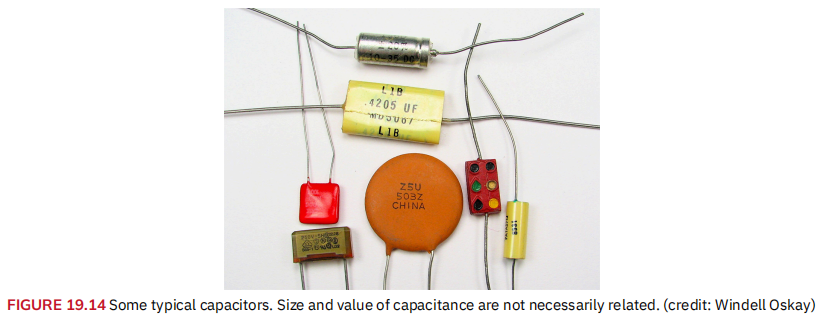
\includegraphics[width=1\linewidth]{phys12-circuits-capacitor-types.png}
    \end{figure}
\end{frame}

\begin{frame}
   \begin{figure}
       \centering
       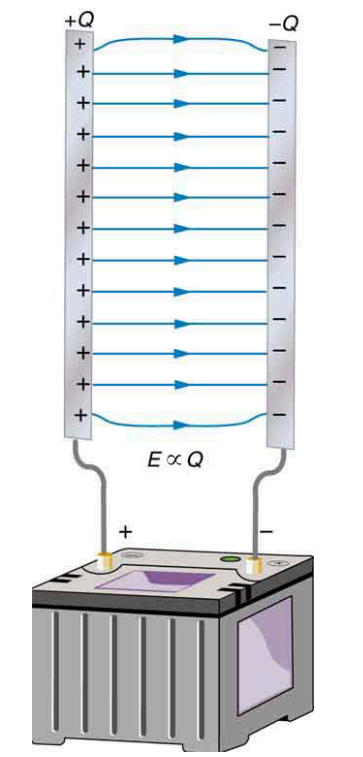
\includegraphics[width=0.3\linewidth]{phys12-circuits-capacitor-symbol.png}
       \caption{fig 19.13}
   \end{figure}
\end{frame}

\begin{frame}
    \frametitle{Capacitance}
    
    \begin{block}{Capacitance Definition}
        Capacitance (C) is the amount of charge stored per volt of potential difference:
        \begin{align}
            C = \frac{Q}{V}
        \end{align}
    \end{block}
    
    \begin{itemize}
        \item Unit: Farad (F), where 1 F = 1 C/V
        \item Typical values: pF to μF range
        \item Depends only on physical characteristics (geometry, materials)
        \item Does NOT depend on charge or voltage (for linear capacitors)
    \end{itemize}
\end{frame}

\begin{frame}
    \frametitle{Parallel Plate Capacitor}
    
    \begin{block}{Capacitance Formula}
        The capacitance of a parallel plate capacitor in a vacuum or air:
        \begin{align}
            C = \epsilon_0 \frac{A}{d}
        \end{align}
        where:
        \begin{itemize}
            \item $\epsilon_0 = 8.85 \times 10^{-12}$ F/m (permittivity of free space)
            \item $A$ = area of plates
            \item $d$ = separation distance between plates
        \end{itemize}
    \end{block}
    
    \begin{itemize}
        \item Larger plate area → greater capacitance
        \item Smaller separation → greater capacitance
    \end{itemize}
\end{frame}

\begin{frame}
    \frametitle{Dielectrics in Capacitors}
    
    \begin{block}{Effect of Dielectrics}
        Inserting a dielectric material between capacitor plates:
        \begin{align}
            C = \kappa\epsilon_0 \frac{A}{d}
        \end{align}
        where $\kappa$ is the dielectric constant of the material
    \end{block}
    
    \begin{block}{Common Dielectric Constants}
        \begin{itemize}
            \item Air: $\kappa \approx 1.00059$
            \item Paper: $\kappa \approx 2-4$
            \item Glass: $\kappa \approx 4-10$
            \item Teflon: $\kappa \approx 2.1$
            \item Water: $\kappa \approx 80$
        \end{itemize}
    \end{block}
    
 
\end{frame}

\section{Capacitors in Series and Parallel}

\begin{frame}
    \frametitle{Capacitors in Series}
    
    \begin{block}{Series Combination}
        When capacitors are connected in series:
        \begin{align}
            \frac{1}{C_S} = \frac{1}{C_1} + \frac{1}{C_2} + \frac{1}{C_3} + \cdots
        \end{align}
    \end{block}
    
    \begin{itemize}
        \item All capacitors in series have the same charge magnitude
        \item The total voltage is divided among the capacitors
        \item Equivalent capacitance is less than any individual capacitance
        \item Similar to resistors in parallel
    \end{itemize}
    
    \begin{center}
        \begin{figure}
            \centering
            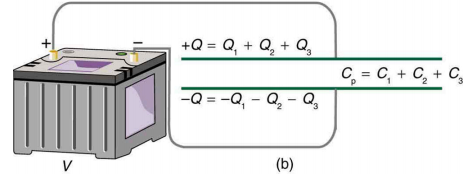
\includegraphics[width=0.3\linewidth]{phys12-circuits-capacitor-in-series.png}
        \end{figure}
    \end{center}
\end{frame}

\begin{frame}
    \frametitle{Capacitors in Parallel}
    
    \begin{block}{Parallel Combination}
        When capacitors are connected in parallel:
        \begin{align}
            C_P = C_1 + C_2 + C_3 + \cdots
        \end{align}
    \end{block}
    
    \begin{itemize}
        \item All capacitors in parallel have the same voltage
        \item The total charge is divided among the capacitors
        \item Equivalent capacitance is greater than any individual capacitance
        \item Similar to resistors in series
    \end{itemize}
    
    \begin{center}
   
      \begin{figure}
          \centering
          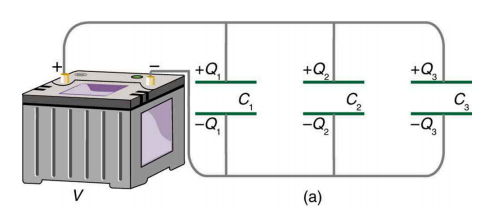
\includegraphics[width=0.5\linewidth]{phys12-circuits-capacitors-in-parallel.png}
      \end{figure}
    \end{center}
\end{frame}

\begin{frame}
    \frametitle{Combined Series-Parallel Networks}
    
    \begin{block}{Strategy for Solving Combined Networks}
        \begin{enumerate}
            \item Identify series and parallel parts in the circuit
            \item Compute the equivalent capacitance for each part
            \item Combine the results to find the total capacitance
        \end{enumerate}
    \end{block}
    
    \begin{center}
 \begin{figure}
        \centering
        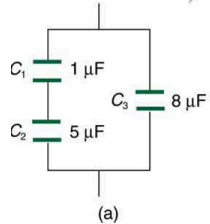
\includegraphics[width=0.3\linewidth]{phys12-circuits-series-parallel-capacitor-combo.png}
    \end{figure}
    
        
    \end{center}
\end{frame}

\section{Energy Stored in Capacitors}

\begin{frame}
    \frametitle{Energy Storage in Capacitors}
    
    \begin{block}{Energy Formula}
        The energy stored in a capacitor can be expressed in three equivalent ways:
        \begin{align}
            E_{cap} &= \frac{QV}{2} \\
            E_{cap} &= \frac{CV^2}{2} \\
            E_{cap} &= \frac{Q^2}{2C}
        \end{align}
    \end{block}
    
    \begin{itemize}
        \item Energy is stored in the electric field between the plates
        \item Units: joules (J)
        \item Work must be done to charge a capacitor
        \item The stored energy can be recovered when the capacitor discharges
    \end{itemize}
\end{frame}

\begin{frame}
    \frametitle{Applications of Capacitors}
    
    \begin{block}{Common Applications}
        \begin{itemize}
            \item Energy storage (backup power supplies)
            \item Filtering in power supplies
            \item Timing circuits
            \item Coupling and decoupling in electronic circuits
            \item Flash lamps in cameras
            \item Defibrillators in medical equipment
            \item Touch screens and sensors
        \end{itemize}
    \end{block}
    
    \begin{block}{Energy Density}
        The energy density in a capacitor's electric field is:
        \begin{align}
            u = \frac{1}{2}\epsilon_0 E^2 \quad \text{(J/m³)}
        \end{align}
    \end{block}
\end{frame}

\section{Example Problems}

\begin{frame}
    \frametitle{"I Do" Example - Electron Acceleration}
    
    \begin{block}{Problem}
        An evacuated tube uses an accelerating voltage of 40 kV to accelerate electrons to hit a copper plate and produce X-rays. What would be the maximum speed of these electrons? (Non-relativistic calculation)
    \end{block}
    
    \begin{block}{Solution}
        Use energy conservation: electrical potential energy is converted to KE
        \begin{align}
            qV &= \frac{1}{2}mv^2 \\
            v &= \sqrt{\frac{2qV}{m}} \\
            v &= \sqrt{\frac{2(1.6 \times 10^{-19} \text{ C})(4.0 \times 10^4 \text{ V})}{9.11 \times 10^{-31} \text{ kg}}} \\
            v &= 1.17 \times 10^8 \text{ m/s}
        \end{align}
    \end{block}
\end{frame}

\begin{frame}
    \frametitle{"We Do" Example - Capacitor with Dielectric}
    
    \begin{block}{Problem}
        A parallel plate capacitor has plates of area 5.00 m² separated by 0.100 mm of Teflon (dielectric constant κ = 2.1). What is the capacitance?
    \end{block}
    
    \begin{block}{Solution}
        Use the formula for a parallel plate capacitor with a dielectric:
        \begin{align}
            C &= \kappa\epsilon_0 \frac{A}{d} \\
            C &= (2.1)(8.85 \times 10^{-12} \text{ F/m})\frac{5.00 \text{ m}^2}{0.100 \times 10^{-3} \text{ m}} \\
            C &= (2.1)(8.85 \times 10^{-12} \text{ F/m})(5.00 \times 10^4 \text{ m}) \\
            C &= 9.29 \times 10^{-7} \text{ F} = 0.929 \text{ μF}
        \end{align}
    \end{block}
\end{frame}

\begin{frame}
    \frametitle{"You Do" Example - Energy in a Capacitor}
    
    \begin{block}{Problem}
        A 180 μF capacitor is charged to 120 V. 
        \begin{enumerate}
            \item How much charge is stored in the capacitor?
            \item How much energy is stored in the capacitor?
        \end{enumerate}
    \end{block}
    
    \begin{block}{Hints}
        \begin{itemize}
            \item Use $Q = CV$ to find the charge
            \item Use $E_{cap} = \frac{1}{2}CV^2$ to find the energy
            \item Pay attention to the units ($μF = 10^{-6} F$)
        \end{itemize}
    \end{block}
    
    Try solving this problem on your own!
\end{frame}

\begin{frame}
    \frametitle{Summary}
    
    \begin{block}{Key Concepts}
        \begin{itemize}
            \item Electric potential: $V = \frac{PE}{q}$
            \item Potential difference: $\Delta V = \frac{\Delta PE}{q}$
            \item Electric field in a uniform field: $E = \frac{V}{d}$
            \item Electric field and potential relationship: $E = -\frac{\Delta V}{\Delta s}$
            \item Point charge potential: $V = k\frac{Q}{r}$
            \item Capacitance: $C = \frac{Q}{V}$
            \item Parallel plate capacitor: $C = \kappa\epsilon_0 \frac{A}{d}$
            \item Series capacitors: $\frac{1}{C_S} = \frac{1}{C_1} + \frac{1}{C_2} + \cdots$
            \item Parallel capacitors: $C_P = C_1 + C_2 + \cdots$
            \item Energy stored: $E_{cap} = \frac{1}{2}CV^2$
        \end{itemize}
    \end{block}
\end{frame}

\end{document}